\documentclass[10pt,portrait, twocolumn]{article}
\usepackage{multicol}
\usepackage{calc}
\usepackage[portrait]{geometry}
\usepackage{amsmath,amsthm,amsfonts,amssymb}
\usepackage{times}
\usepackage{color,graphicx,overpic}
\graphicspath{ {images/} }
\usepackage{hyperref}
\usepackage{pgfplots}
\usepackage{esint}
\usepackage{bm}
\usepackage{tikz}
\usepackage{relsize}
\usepackage{datetime}
\usepackage[utf8] {inputenc}
\usepackage[spanish, activeacute] {babel}
\usepackage{IEEEtrantools}
\usepackage{framed}

\usepackage{pdflscape}

\usepackage{draftwatermark}
\SetWatermarkText{Javier de Martín}
\SetWatermarkScale{0.8}

% This sets page margins to .5 inch if using letter paper, and to 1cm
% if using A4 paper. (This probably isn't strictly necessary.)
% If using another size paper, use default 1cm margins.
\geometry{top=.5cm,left=.5cm,right=.5cm,bottom=.5cm}
    
\pgfplotsset{
    dirac/.style={
        mark=triangle*,
        mark options={scale=2},
        ycomb,
        scatter,
        visualization depends on={y/abs(y)-1 \as \sign},
        scatter/@pre marker code/.code={\scope[rotate=90*\sign,yshift=-2pt]}
    }
}

% Turn off header and footer
\pagestyle{empty}

% Redefine section commands to use less space
\makeatletter
\renewcommand{\section}{\@startsection{section}{1}{0mm}%
                                {-1ex plus -.5ex minus -.2ex}%
                                {0.5ex plus .2ex}%x
                                {\normalfont\large\bfseries}}
\renewcommand{\subsection}{\@startsection{subsection}{2}{0mm}%
                                {-1explus -.5ex minus -.2ex}%
                                {0.5ex plus .2ex}%
                                {\normalfont\normalsize\bfseries}}
\renewcommand{\subsubsection}{\@startsection{subsubsection}{3}{0mm}%
                                {-1ex plus -.5ex minus -.2ex}%
                                {1ex plus .2ex}%
                                {\normalfont\small\bfseries}}
\makeatother

\newcommand{\Lagr}{\mathcal{L}}

% Define BibTeX command
\def\BibTeX{{\rm B\kern-.05em{\sc i\kern-.025em b}\kern-.08em
    T\kern-.1667em\lower.7ex\hbox{E}\kern-.125emX}}

% Don't print section numbers
\setcounter{secnumdepth}{0}


\setlength{\parindent}{0pt}
\setlength{\parskip}{0pt plus 0.5ex}

%My Environments
\newtheorem{example}[section]{Example}
% ---------------------------------------------------------------

\begin{document}


\begin{framed}
	\begin{center}
    	\Large{\underline{Redes de Transporte}} \\
    	\scriptsize{3º Ingeniería de Telecomunicaciones | UPV/EHU}\\
     	%Actualizado por última vez el \today \\
     	"\textsl{Under-promise and over-deliver}." \\
     	%\hspace{5 pt} \\
     	\small{\textbf{Javier de Martín -- 2016}}
	\end{center}
\end{framed}

%%%%%%%%%%%%%%%%%%%%%%%%%%%%%%%%%%%%%%%%%%%%%%%%%%%%%%%%%%%%%%%%%
% Tema 4

\begin{center}
\section{\underline{0.- Introducción}}
\end{center}

Las redes de \textbf{acceso} hacen llegar la información del origen al primer equipo de red. Las redes de \textbf{transporte} llevan la información a través de la red, realiza las tareas de conmutación (nivel 2) y encaminamiento (nivel 3), transmisión y señalización.

\hrulefill

\section{\underline{1.- Encaminamiento}}

\textbf{Encaminar} consiste en establecer una ruta óptima para una instancia de comunicación desde una fuente a un destino. La ruta elegida debe optimizar en lo posible algún parámetro o conjunto de ellos. Las decisiones de encaminamiento son incrementales, cada nodo sólo debe decidir a qué nodo adyacente debe transmitir los datos.

\begin{itemize}
	\item \textbf{Algoritmo de encaminamiento}: Dado un destino decide la línea de salida adecuada.
	\item \textbf{Tabla de encaminamiento}: Estructura de información donde almacenar localmente los pares destino-salida.
	\item \textbf{Protocolo de encaminamiento}: Coordinación entre nodos del cálculo de las rutas e informar de entre sí de los cambios que se produzcan, por ejemplo, en la topología de la red.
\end{itemize}

Los encaminamientos deben de ser \textbf{robustos} para adaptarse a los posibles cambios de topología sin necesidad de abortar o reiniciar la red, \textbf{estables} en el sentido de converger a un resultado lo más rápido posible, no deben de generar \textbf{bucles} en el encaminamiento y no deben \textbf{favorecer} a ningún usuario frente a otro sin motivo.

\subsection{Encaminamiento IP}

En función de \textbf{dónde se decide encaminar}:

	\begin{itemize}
		\item \textbf{Fijado en el origen (Source Routing)}: Son los sistemas finales los que fijan la ruta que ha de seguir cada paquete. Cada paquete lleva un campo que especifica su ruta (RI, Routing Information), y los nodos sólo se dedican a reenviar los paquetes por esas rutas ya especificadas. Los sistemas finales son los que tienen las tablas de encaminamiento y no se hace necesaria la consulta o existencia de tablas de encaminamiento en los nodos intermedios. El nodo origen debe de conocer la topología de la red. No existen bucles, el sistema final fija la ruta.
		\item \textbf{Salto a Salto (Hop by Hop)}: Los nodos, en función del destino, conocen sólo el siguiente salto a realizar. Pueden ocurrir bucles, no se tiene una visión completa de la red.
	\end{itemize}
	
En función de la \textbf{adaptabilidad}:

	\begin{itemize}
		\item \textbf{No adaptables (estáticos)}:
			\begin{itemize}
				\item Estáticos: Las tablas de encaminamiento de los nodos se configuran de forma manual y permanecen inalterables hasta que no se vuelve a actuar sobre ellas. Tanto la recogida como la distribución de información se realiza por gestión (manera externa a la red), sin ocupar capacidad de red. Es óptimo para topologías de red en las que sólo hay una posibilidad de encaminamiento (topología en estrella).
				\item Q-Estáticos: Igual que el estático pero en vez de dar una sola ruta fija se proporcionan varias alternativas en caso de que la principal no funcione. Tiene adaptabilidad reducida.
			\end{itemize}
		\item \textbf{Adaptables (dinámicos)}:
			\begin{itemize}
				\item Centralizados: Los nodos envían a un nodo central la información de control acerca de sus vecinos. El nodo central será el que se encargue de recoger esta información de control acerca de sus vecinos. El nodo central será el que se encargue de recoger esta información para construir la tabla de encaminamiento de cada nodo en función de la información de control que éstos le mandan. Tiene un alto consumo de recursos de la red y se necesita disponer de rutas alternativas (y nodo central alternativo) para comunicarse con el nodo central, ya que estos métodos dejarían de funcionar con la caída de éste.
				\item Aislados: El más simple, no tiene en cuenta la información de los otros nodos a la hora de encaminar. Cada vez que un nodo recibe un paquete que tiene que reenviar (porque no es para él) lo reenvía por todos los enlaces salvo por el que le llegó (inundación). Útil para enviar información de emergencia ya que se asegura que llega a todos los nodos.
				\item Distribuidos: Todos los nodos son iguales, todos envían y reciben información de control y todos calculan, a partir de su RIB (base de información de encaminamiento) sus tablas de encaminamiento. La adaptación a cambios es óptima siempre y cuando éstos sean notificados.
			\end{itemize}
	\end{itemize}

\begin{center}
\begin{tabular}{|l|l|l|l|}
\hline
\textbf{Encaminamiento} & \textbf{Info de Control} & \textbf{Decisión} & \textbf{Adaptación} \\ \hline
\textbf{Estáticos}               & No                              & Offline                             & No                                \\ \hline
\textbf{Cuasiestáticos}          & No                              & Offline                             & Reducida                          \\ \hline
\textbf{Centralizado}            & Nodo Central                    & Nodo Central                        & Si                                \\ \hline
\textbf{Distribuido}             & Entre Nodos                     & Cada Nodo                           & Si                                \\ \hline
\textbf{Aislado}                 & no                              & Cada Nodo                           & Si                                \\ \hline
\end{tabular}
\end{center}

En el encaminamiento \textbf{estático} la tabla de encaminamiento de los equipos se actualiza de forma manual y en el \textbf{dinámico} se actualiza mediante protocolos de encaminamiento.

\subsection{Encaminadores o Routers}

Un \textbf{router} tiene que encontrar una ruta y encaminar los datos. \textit{Routing} es el proceso de decidir a dónde enviar un paquete recibido utilizando la tabla de encaminamiento del router y \textit{forwarding} es el acto de enviar el paquete al siguiente salto.\\

Los routers tienen dos tablas clave:

	\begin{itemize}
		\item \textbf{FIB} (Forwarding table): Contiene destinos y las interfaces para llegar a ellos. El router la utilizar para descubrir la interfaz a la que enviar los paquetes. A veces se confunden con rutas (\textbf{no entiendo esto}).
		\item \textbf{RIB} (Routing table): Contiene una lista de los destinos alcanzables y los siguientes saltos para alcanzar los destinos. Un destino puede ser alcanzado a través de varios posibles next hops pero sólo el mejor va a la FIB.
	\end{itemize}
	
	\begin{center}
		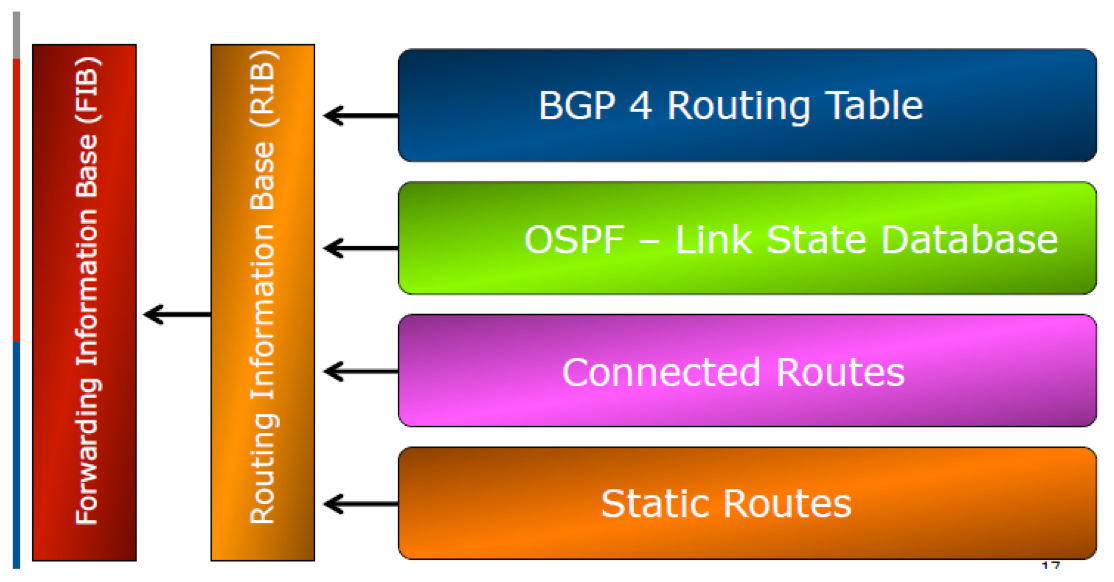
\includegraphics[scale = .5]{FIBRIB}
	\end{center}
	
\subsection{Encaminamiento IP}

El protocolo IP es un protocolo \textbf{no fiable} (best effort), \textbf{no orientado a conexión}, no mantiene \textbf{información de estado}, los datagramas pueden llegar fuera de secuencia con errores o pérdidas, es el protocolo de nivel superior el encargado de resolver estos problemas. \\

IP realiza tiene dos tipos de encaminamiento:

	\begin{itemize}
		\item \textbf{Directo}: Un equipo puede enviar un paquete IP a otra máquina sin pasar por un tercer equipo. En la misma red.
		\item \textbf{Indirecto}: Un equipo quiere enviar un paquete IP a otro equipo y tiene que atravesar una ruta de otros equipos. En distintas redes.
	\end{itemize}

La tabla de encaminamiento IP en cada equipo incluye un conjunto de direcciones IP destino y las direcciones IP del siguiente salto para cada destino. Además, pueden incluir para llegar a destinos rutas directas, indirectas o por defecto. \\

El algoritmo de encaminamiento IP es el siguiente:
	\begin{center}
		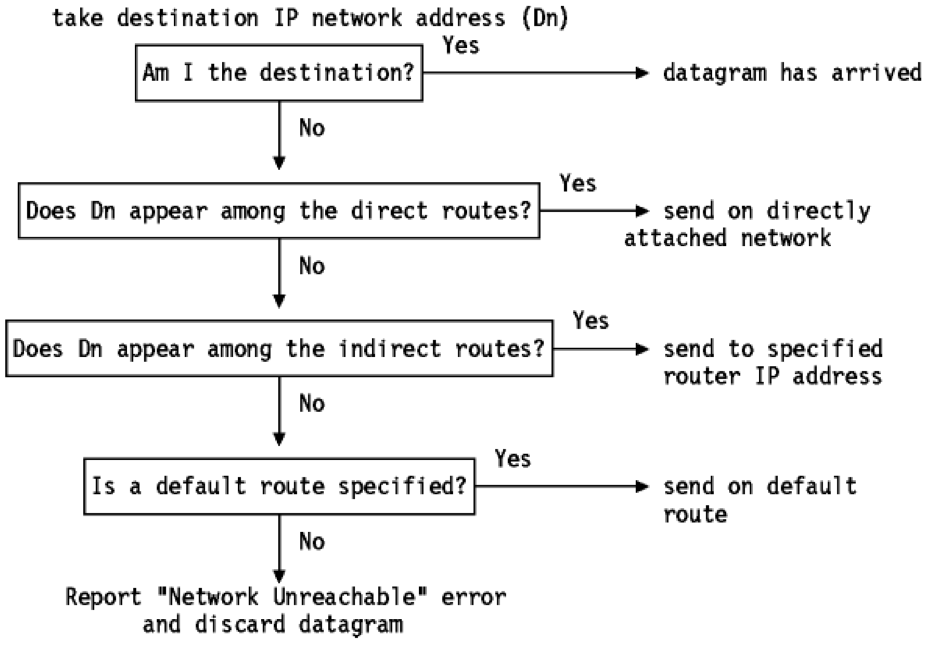
\includegraphics[scale = .5]{AlgoritmoIP}
	\end{center}

\subsection{Encaminamiento en Internet}

Para entender el encaminamiento en internet hay que conocer algunos \textbf{aspectos clave}.  La transmisión es \textbf{no orientada a conexión}, cada router toma decisiones de forma \textbf{local} para encaminar los paquetes hasta el destino. Internet no es una única red sino una colección de reds interconectadas perteneciente a distintos propietarios. Internet se divide en \textbf{Sistemas Autónomos} que está formado por routers, equipos y redes gestionados por una misma administración. Cada Sistema Autónomo se identifica mediante un AS Number que es de 32 bits (antiguamente de 16) y es asignado por las autoridades de numeración de Internet. La división de Internet en Sistemas Autónomos tiene ventajas como la autonomía, disminuye los \textit{overheads} derivados de operaciones de control (encaminamiento), facilita la gestión de las redes...

Los \textbf{protocolos de encaminamiento} permiten la actualización de información de forma dinámica intercambiando información. Hay dos tipos de protocolos de encaminamiento:

	\begin{itemize}
		\item \textbf{IGP} (Interior Gateway Protocol): Operan dentro de un Sistema Autónomo (intra-domain routing), los mensajes IGP se intercambian entre routers que pertenecen a un mismo SA. Cada SA, normalmente, tendrá su propia política de encaminamiento.
		\item \textbf{EGP} (Exterior Gateway Protocol): (inter-domain routing) Permiten intercambio de información entre Sistemas Autónomos.
	\end{itemize}
	
	\begin{itemize}
		\item \textbf{Intradomain Routing}: Encaminamiento dentro de un AS. No tiene en cuenta lo que hay, Internet, fuera del propio AS.
		\item \textbf{Interdomain Routing}: Encaminamiento entre AS. Considera Internet como un conjunto de AS interconectados. Normalmente hay un router en cada AS que maneja tráfico interdomain.
	\end{itemize}
	
	\begin{center}
		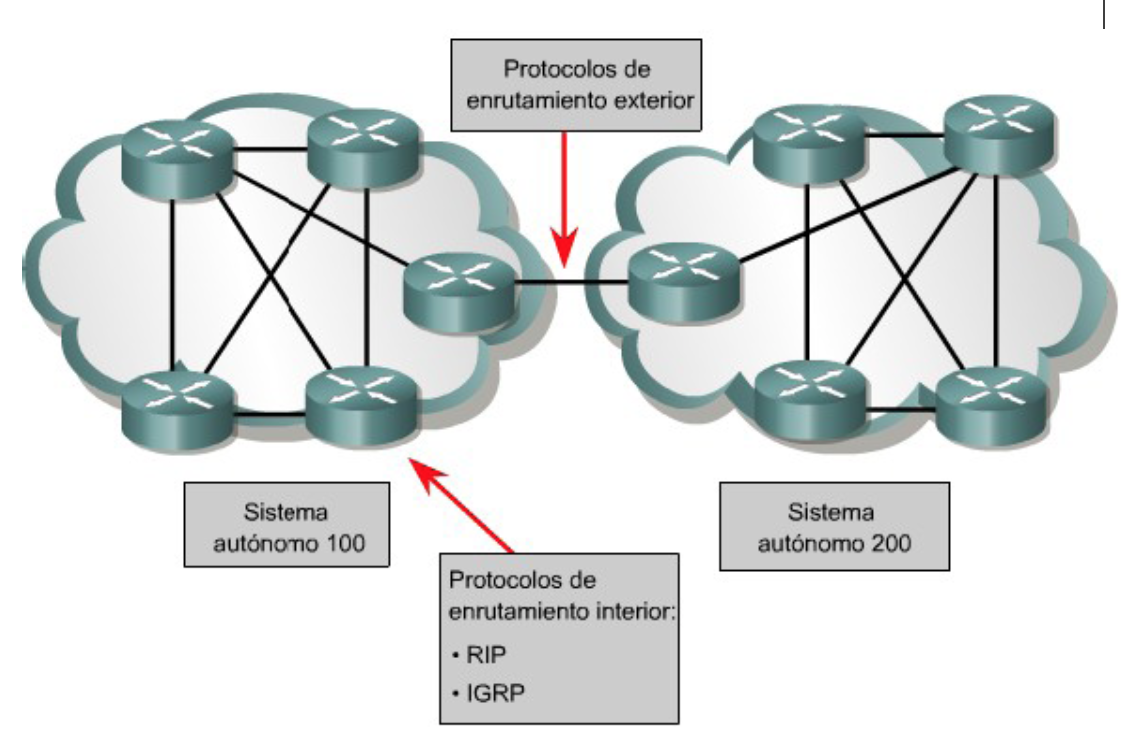
\includegraphics[scale = .5]{InterIntra}
	\end{center}
	
El \textbf{encaminamiento IGP} en redes actuales suele basarse en una combinación de protocolos de encaminamiento dinámicos y rutas estáticas. Cada escenario (parte de una red) tiene diferentes requerimientos. El \textbf{encaminamiento estático} es adecuado cuando hay pocas alternativas (rutas) para elegir que no cambian mucho, por ejemplo cuando un router conecta a una red a Internet o habitual en equipos finales. En equipos IP normalmente consiste en introducir manualmente \texttt{IP address/subnet mask + gateway}. Los protocolos de \textbf{encaminamiento dinámico} comparten la información entre routers, actualizan los encaminamientos cuando se producen cambios en la topología (cambio de rutado), determinan la mejor ruta a cada destino, aprenden información de nuevas redes y destinos y encuentran rutas alternativas en caso de fallos. Sus \textbf{componentes}:

	\begin{itemize}
		\item Estructuras de datos
		\item Algoritmos
		\item Mensajes de Protocolo
		\item Terminar
	\end{itemize}
	
\textbf{Ventajas} rutado estático:
	\begin{itemize}
		\item Mínimo procesado de CPU.
		\item Fácil de entender y administrar.
		\item Fácil de configurar
		\item No requiere recursos extra
		\item Más seguro 
	\end{itemize}
	
\textbf{Desventajas} rutado estático:

	\begin{itemize}
		\item Los cambios en la red requieren reconfiguración manual.
		\item La configuración y mantenimiento son time-consuming.
		\item No escala bien en topologías grandes.
		\item Configuraciones error-prone, especialmente en redes grandes.
	\end{itemize}

\textbf{Ventajas} rutado dinámico:

	\begin{itemize}
		\item El administrado rtiene menos tareas de configuración cuando se añaden o quitan redes nuevas.
		\item Los protocolos reaccionan automáticamente ante cambios de la topología.
		\item La configuración es menos error-prone.
		\item Más escalable.
	\end{itemize}

\textbf{Desventajas} rutado dinámico:

	\begin{itemize}
		\item Uso de recursos de los routers.
		\item Se requieren más conocimientos de administración de red...
	\end{itemize}
	
Tipos de protocolos de encaminamiento IGP (Interior Gateway Protocol) se dividen en dos grupos grandes:

	\begin{itemize}
		\item Distance Vector Routing Protocols: RIPv1 y IGRP.
		\item Link-State Routing Protocols: OSPF, IS-IS.
	\end{itemize}

Cuando se selecciona un protocolo para un caso u otro  hay que fijarse en ciertos criterios: como el tiempo de convergencia, escalabilidad, utilización de recursos, implementación y mantenimiento...\\

Hay que entender un concepto clave, la \textbf{métrica} es el coste asociado a una ruta. Los protocolos utilizan métricas para evaluar, diferenciar y seleccionar entre rutas a destinos. Cada protocolo utiliza distintos tipos de métricas. Hay protocolos que soportan la utilización de varias métricas a la vez. También se pueden configurar costes de forma manual. La métrica total de una ruta es igual a la suma de métricas de todos los enlaces (redes) que componen la ruta.\\

Los algoritmos de vector distancia se basan en el algoritmo de Bellman-Ford para calcular la mejor ruta al destino. Los routers no tienen información completa sobre la topología de la red, sólo conocen la interfaz de salida o dirección del siguiente router para cada destino. Suelen hacer envíos periódicos de vectores distancia a todos los vecinos conectados. \textbf{Funcionamiento}, cada router conoce a sus vecinos y sus enlaces hasta los vecinos. Cada router envía información de su tabla de encmainamiento que se anuncia como vectores de pares.

SALTO HASTA LA PAGINA 30

La \textbf{convergencia} es el estado de una red cuando las tablas de encaminamiento de los routers son consistentes. El \textbf{tiempo de convergencia} es el tiempo que transcurre cuando los routers intercambian información de sus tablas de encaminamiento, calculan las mejores rutas a los destinos, actualizan las tabals de encaminamiento (si es necesario) y construyen y envían los correspondientes VD si es necesario. Es un parámetro importante para caracterizar los protocolos de encaminamiento, cuanto más rápido se alcanza la convergencia mejor es el protocolo de routing.\\

\textbf{¿Cuándo se envían los vectores distancia?} Se hacen actualizaciones periódicas, haciendo algunos protocolos con reconocimiento. Triggered updates, los nodos envían vectores cuando detectan algún cambio en su tabla de encaminamiento después de una actualización por recepción de VD o cuando detectan algún fallo en algún enlace (o enlace nuevo).\\

\textbf{Fallo en un enlace/nodo)}, ¿cómo detectarlo? No llegan los envíos periódicos o una interfaz pasa al estado \texttt{down}. La propagación de la información de nueva topología, el nodo destino cambia la distancia al nodo $X$ a $\infty$ y envía update a sus vecinos (VD), los updates se procesan y reenvían hasta que la red converge.\\

Para los algoritmos de VD hay un problema, el \textbf{count to infitity}. Un nodo se inutiliza y el adyacente envía el $\infty$ de actualización a sus vecinos pero se pierde. TERMINAR\\

Como solución a Count to Infinity se propone \textbf{Split Horizon}. Consiste en no enviar información por la interfaz por la que se recibió, se envían diferentes versiones de VD. COPIAR IMAGENES

Los algoritmos de vector distancia tienen los siguientes \textbf{problemas}: \textbf{Convergencia lenta} que se soluciona con triggered updates y son \textbf{inestables} que se soluciona con la representación de la no alcanzabilidad mediante valor infinito (limitando el tamaño de las rutas) o Split Horizon (no evita todos los bucles, solo los de dos saltos).\\

El \textbf{propósito de los algoritmos VD} es enviar recibir updates, calcular mejores rutas (instalar rutas en su TE) y detectar y reaccionar ante cambios en la topología. Los algoritmos VD se caracterizan por ser un proceso iterativo y distribuido. COPIATR GRAFICO

TABLA VENTAJAS Y DESVENTAJAS

\textbf{Ejemplos} de protocolos de encaminamiento VD: RIP, IGRP y EIGRP.

\textbf{Conclusiones RIP}: Es muy simple y por eso muy utilizado, si la red es simple y los fallos no muy frecuentes su resultado es aceptable pero para redes grandes y complejas noe s muy adecuado ya que clcula nuevas rutas después de cada cambio en la topología pudiendo provocar cuentas hasta infinito o generar bucles que provocan congestiones.


\subsection{Bloque 3. Encaminamiento}

\hrulefill

\textbf{Algoritmo Link State} surge del estudio de la conveniencia de calcular encaminamientos de formacentralizada o distribuida. Conocido también como algoritmos SPF (\textit{Shortest Path First}). Basado en algoritmos SPF de Dijkstra. En los protocolos del estado del enlace, todos los nodos mantienen un mapa de la red: las mejores rutas se calculan de forma independiente en cada nodo en base al mapa. El mapa se mantiene en una base de datos en la que cada entrada representa un en lace de la red. Con la información de la BD, cualquier nodo puede calcular el camino más corto hasta otros nodos. Como todos los nodos tienen la misma información en la BD, las rutas serán coherentes y \textbf{no formarán bucles}.

\begin{figure}[h]
	\centering
     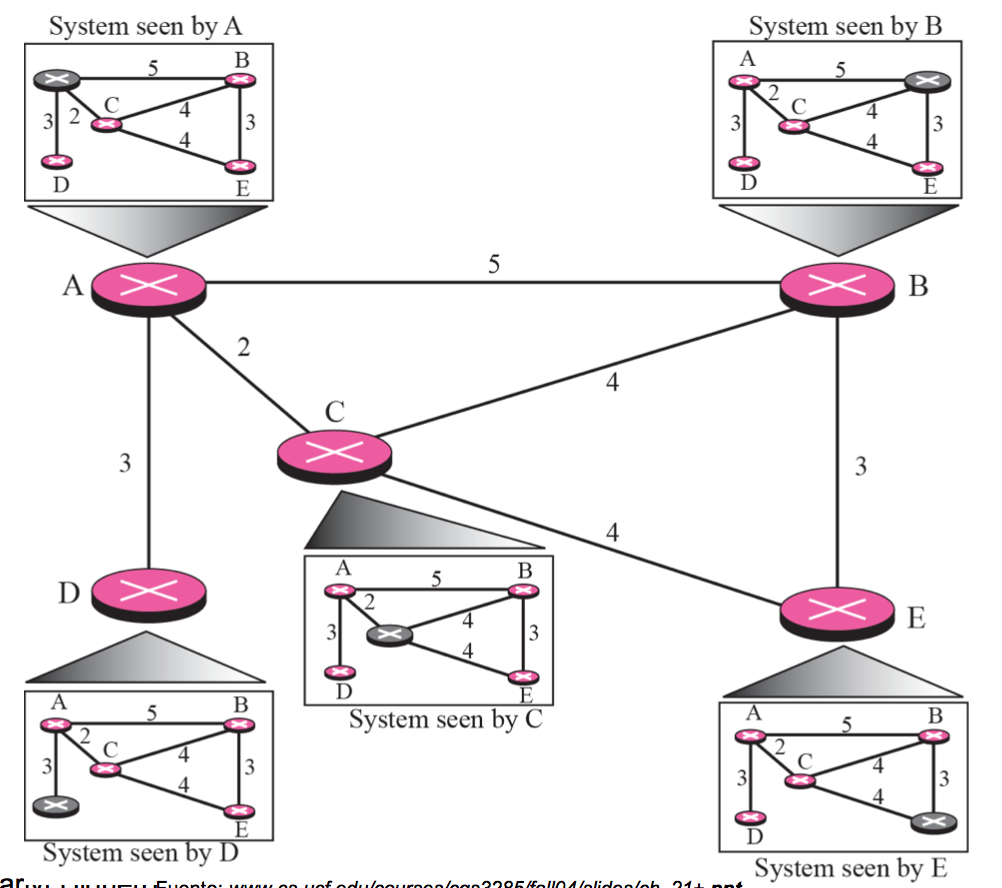
\includegraphics[width=0.3\textwidth]{IGP}
      \caption{Algoritmos Link State}
      \label{fig:Regiones de frecuencias}
  \end{figure}

El \textbf{funcionamiento} de los protocolos Link State, la BD constituye la información que se almacenaría en cada uno de los nodos conteniendo cada entrada:
	
	\begin{itemize}
		\item Identificativo de interfaz (número de enlace).
		\item Información describiendo el estado del enlace (LS): Destino y distancia (métrica)
	\end{itemize}
	
Con esa información cada nodo puede calcular el camino más corto desde él hasta cada nodo. Los cálculos son rápidos.\\

\textbf{¿Cómo logran  la convergencia?} Cada router conoce sus propias redes conectadas directamente. Los routers de estado de enlace intercambian un paquete de saludo para 'conocer' a los routers de estado de enlace conectados directamente. Cada router crea su propio paquete de estado de enlace (LSP) que incluye información sobre los vecinos, como la ID, el tipo de enlace y el ancho de banda. Una vez creado el LSP, el router lo envía a todos sus vecinos que almacenan la información y luego la reenvían hasta que todos los routers tengan la misma información. Cuando todos los routers han recibido los LSP crean un mapa topológico de la red que se utiliza para determinar las mejores rutas para un destino.\\

\textbf{Protocolo de inundación}, para que los encaminamientos puedan adaptarse a las condiciones cambiantes de la red se debe de actualizar la base de datos después de cada cambio en la red. Si dos nodos adyacentes detectan el fallo del enlace actualizarán las entradas correspondientes de la BD construyendo las nuevas TE, transmitirán las nuevas al resto de nodos mediante inundación. Hay que evitar que un mensaje antiguo llegue a corromper la BD, para ello cada mensaje dispone de un número de secuencia o sello de tiempo. \textbf{¿Cómo funciona el mecanismo de inundación?} Se recibe un mensaje y se busca el registro correspondiente en la BD local \footnote{Las actualizaciojnes causan la transmisión del mensaje a través de todas las intefaces excepto por la que llegó el mensaje original}, si el registro existe y el número de la información recibida es mayor que el de la almacenada, actualizar el registro y broadcast del mensaje. Si el registro existe y su número es mayor, transmitir el valor de la BD por la interfaz que llegó el mensaje. Si ambos números son iguales no hacer nada.\\

\textbf{Sincronización de las Bases de Datos} si falla un nodos sólo pueden distribuir información a los vecinos conectados. Cuando termine la inundación existirán dos versiones distintas de la Base de Datos. Este problema, en principio, no tiene importancia. Si las dos mitades separadas mucho tiempo las dos versiones de las BDs evolucionarán independientemente. Establecer conectividad entre dos nodos requiere más que el envío de un registro de la BD, es necesario garantizar la consistencia de las BDs.

Características \textbf{relevantes}:

	\begin{itemize}
		\item Mapa de red actualizado en una base de datos.
		\item Protocolo de inundación para difusión de información
		\item Sincronización de Bases de Datos para alinear las Bases de Datos en los nodos
		\item Algoritmos SPF para cálculos de rutas.
	\end{itemize}
	
\textbf{Conclusiones}:

	\begin{itemize}
		\item Ventajas: Utiliza costes para el cálculo de rutas, convergencia más rápida que protocolos VD y es más escalable soportando división de redes en áreas.
		\item Desventajas: Hace uso de más memorias en los equipos y es más complejo.
	\end{itemize}


\subsubsection{Protocolo OSPF (Open Shortest Path First)}

OSPF es un protocolo de estado del enlace. Viaja sobre IP en las tramas pero requiere mucho procesado y  memoria. En el encendido de la red consume muchos recursos hasta que converge pero luego en estabilidad no consume tanto. Los nodos mantienen un mapa de la red que se actualizará rápidamente ante cualquier cambio. Soporta: BDs distribuidas, procedimiento de inundación, sincronización de las BDs y entradas especiales para rutas externas.\\

Divide la red en \textbf{áreas}. Si el tamaño de una red crece también crecen las BDs, el tiempo de cálculo de las rutas y el volumen de mensajes. En una red grande estos factores pueden ser excesivos. OSPF divide la red en partes independientes interconectadas llamadas áreas unidas mediante un \textbf{área troncal}, cada área se comporta como una red independiente (las BDs sólo contienen info de sus enlaces y mecanismos de inundación hasta la frontera), para poder unir las zonas entre sí algunos routers pertenecen a varias áreas. Se ejecuta sobre IP y tiene tres subprotocolos:

	\begin{itemize}
		\item Protocolo \texttt{Hello}: Comprueba que un enlace está operacional y realiza otras operaciones de control.
		\item Protocolo \texttt{Exange}: Para sincronización inicial de BD.
		\item Protocolo \texttt{Flooding}: Envío de información acerca de actualización de rutas, mantiene sincronizadas las BDs y se utiliza cuando un enlace cambia de estado y en respuesta a una petición.
	\end{itemize}
	
	
\begin{figure}[h]
	\centering
     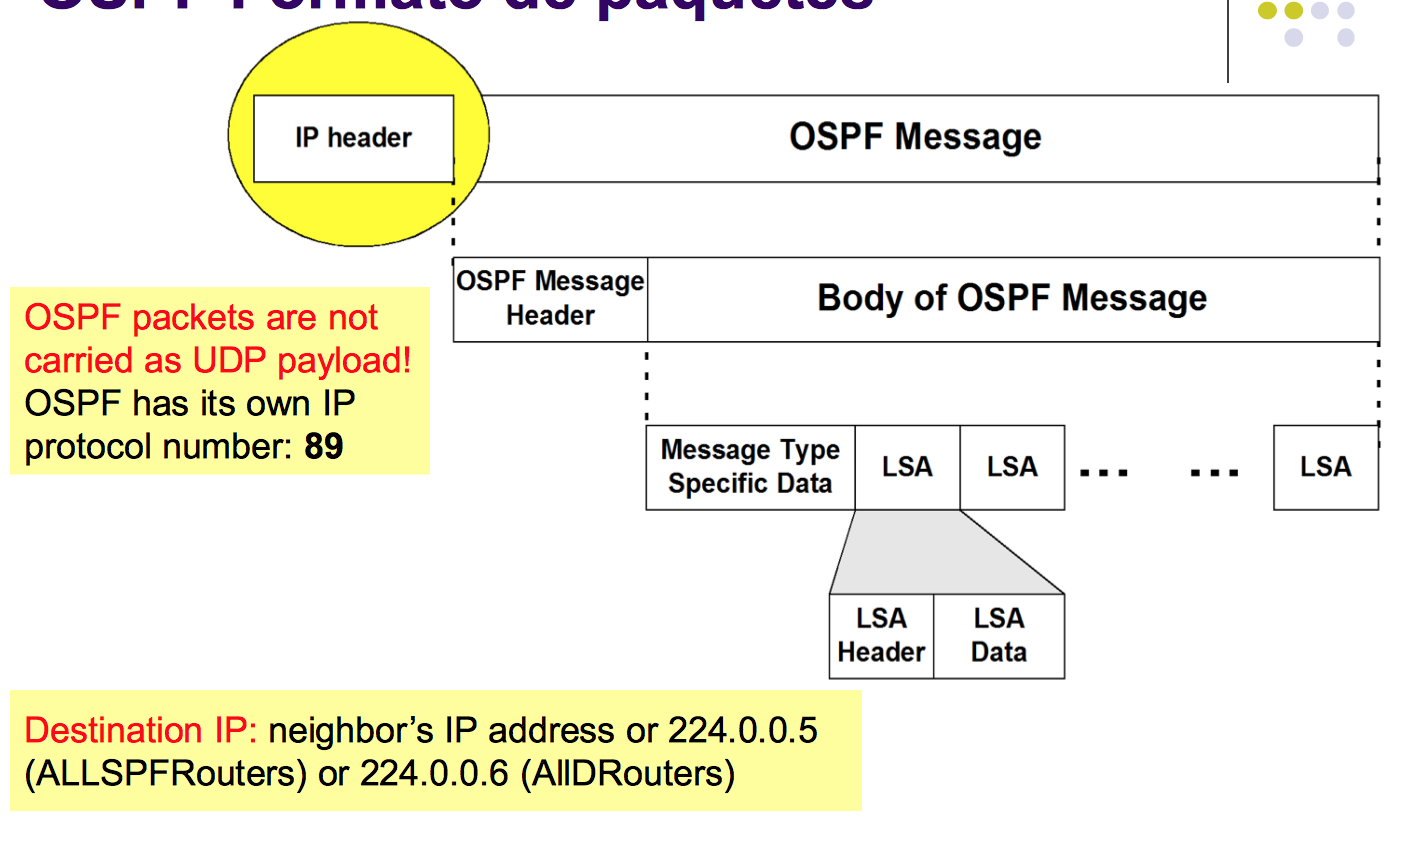
\includegraphics[width=0.4\textwidth]{OSPF}
      \caption{OSPF Formato de Paquetes}
      \label{fig:Regiones de frecuencias}
  \end{figure}
  
\begin{figure}[h]
	\centering
     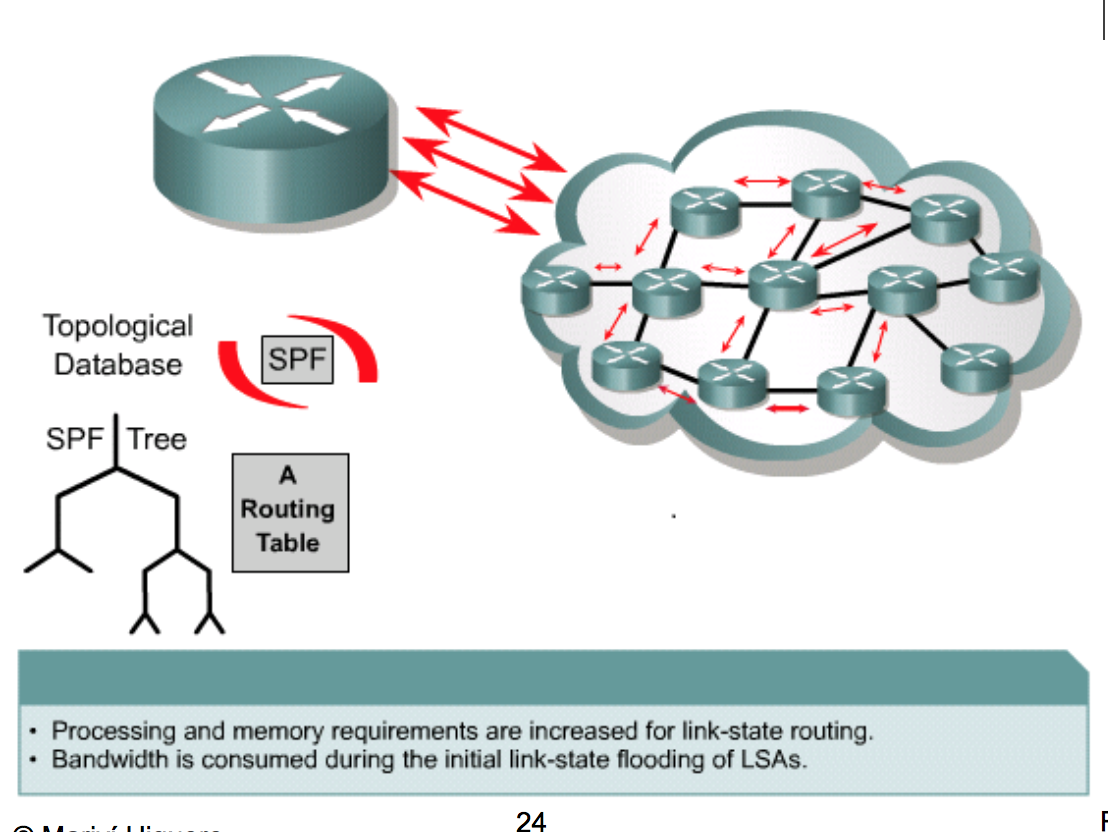
\includegraphics[width=0.4\textwidth]{OSPF2}
      \caption{Protocolo OSPF}
      \label{fig:Regiones de frecuencias}
  \end{figure}
	
\textbf{OSPF vs RIP}:

	\begin{itemize}
		\item OSPF es mucho más complejo que RIP, la gestión requiere una mayor cantidad de información, las implementaciones requieren más código y son más complejas
		\item Requerimientos mayores de los protocolos LS, utilizan más memoria, requieren más CPU y requieren mucho ancho de banda en el startup inicial.
		\item OSPF es más eficiente y utiliza menos mensajes pero es más complejo que RIP.
		\item Distance Vector Routing, cada nodo conoce a sus vecinos directamente conectados, cada nodo sólo conoce distancias a destinos, cada nodo envía periódicamente su tabla de encaminamiento a sus vecinos \footnote{Los updates pueden ser grandes pero sólo viajan por un enlace}. Si todos los nodos envían los updates de sus TE, las tablas de encaminamiento terminan convergiendo.
		\item Lisnk State Routing, cada nodo conoce la distancia a sus vecinos, cada nodo conoce la topología entera. La información de enlaces y distancias se envía a todos los nodos de la ted. Cada nodo calcula las TE de forma independiente.
	\end{itemize}
	
\subsection{Encaminamiento en Internet}

\subsubsection{Protocolos EGP}

\textbf{BGP} (\textbf{Border Gateway Protocol}) es el estándar de facto. Proporciona a cada AS capacidad para:

	\begin{enumerate}
		\item Obtener información de alcanzabilidad de los ASs vecinos.
		\item Propagar la información de alcanzabilidad desde los ASs vecinos.
		\item Determinar rutas 'buenas' a destinos basadas en información de alcanzabilidad y políticas de encaminamiento.
	\end{enumerate}
	
Permite a las subredes anunciar su existencia al resto de Internet. \textbf{Características} de BGP:

	\begin{itemize}
		\item Limitaciones de los protocolos de vector distancia: Toda la información de la ruta se concentra en la métrica y no siempre la ruta más corta es la preferida, es insuficiente para la resolución de bucles.
		\item Si se utilizara un protocolo más potente del estado del enlace puede que no todos los equipos tengan las mismas preferencias. Las técnicas para evitar bucles podrían suponer grandes overheads. Los broadcasts y cálculos de la BD a todo Internet demasiado grandes.
	\end{itemize}

\textbf{Estrategia de rutado} de BGP. \textbf{Path Vector Routing}, toda la información de actualización de encaminamiento llevará la lista completa de SAs recorridos. Se daría un bucle si un AS estuviera listado 2 veces. La protección contra bucles es simple: cuando un SA reciba un anuncio de ruta, el router exterior comprobará que su SA no esté en la lista: si el SA está en la lista el router rechaza emplear esa ruta y si no aparece añadirá su identificativo antes de seguir transmitiendo el anuncio. Ventajas: no requiere que todos los routers utilicen las mismas métricas y si se actualizan los path vector de forma adecuada se asegura que se evitan los bucles.
  
\begin{figure}[h]
	\centering
     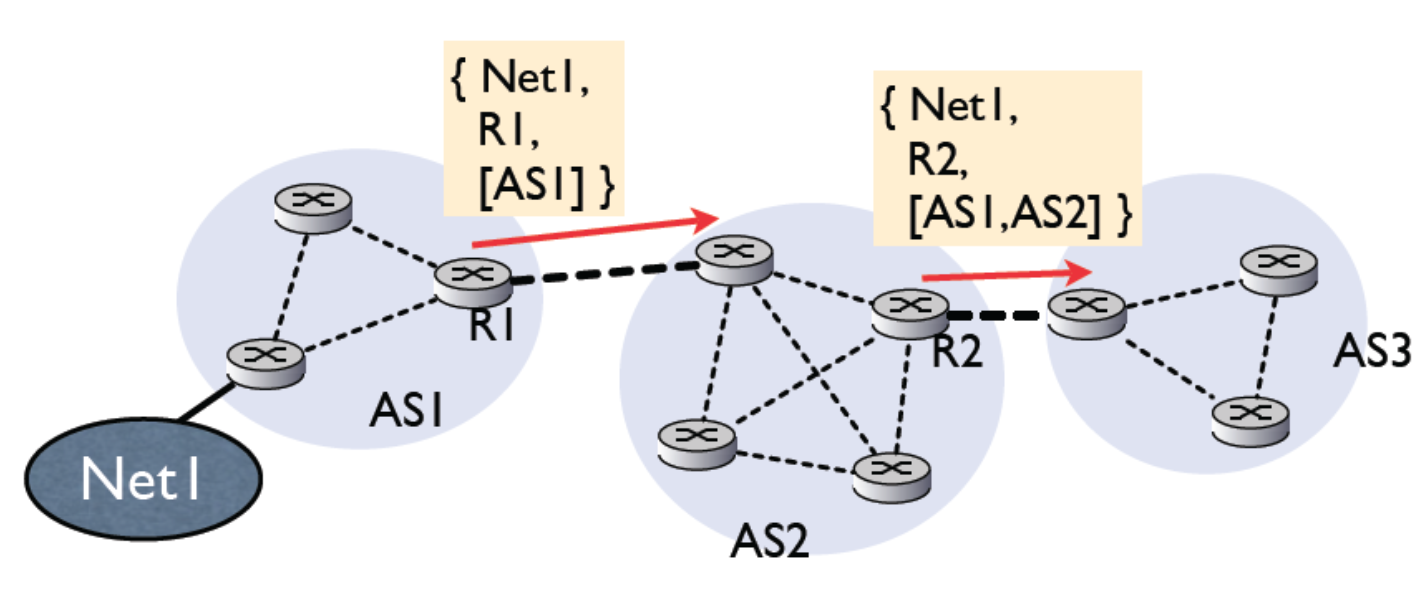
\includegraphics[width=0.4\textwidth]{PathVector}
      \caption{Path Vector}
      \label{fig:Regiones de frecuencias}
  \end{figure}
	
\textbf{Atributos de las rutas}, las rutas se describen mediante un conjunto de atributos, de los cuales los más importantes son: lista de SAs atravesados y lista de redes accesibles. Cuando hay varias rutas disponibles se añaden atributos para facilitar la elección. Formato de los atributos, tripleta de longitud variable:

	\begin{verbatim}
	<attribute type, attribute length, attribute value>
	\end{verbatim}

\begin{figure}[h]
	\centering
     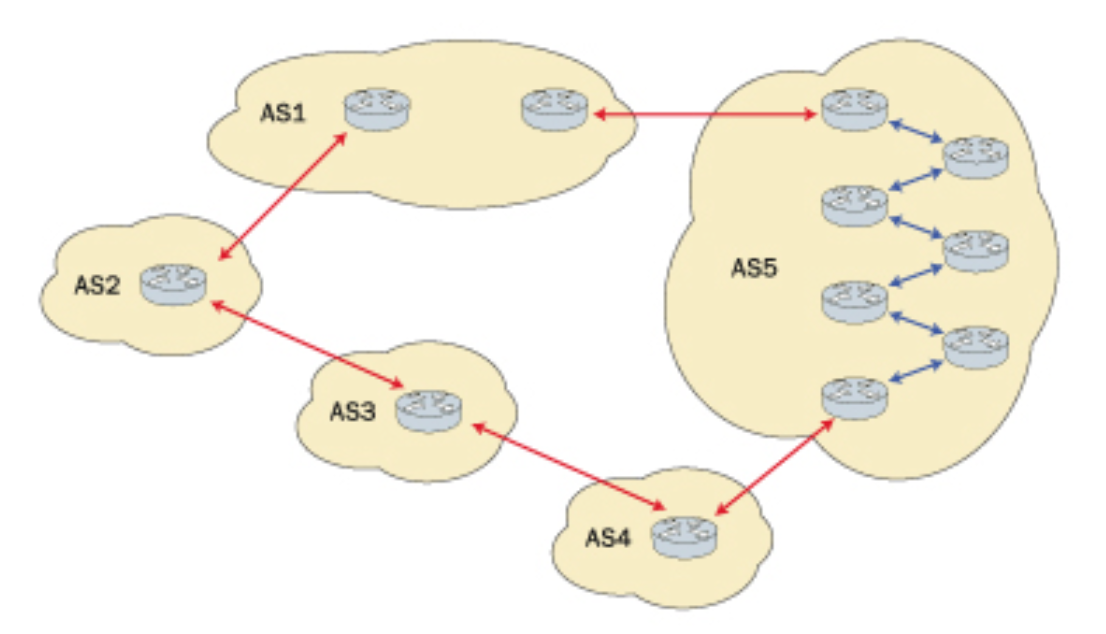
\includegraphics[width=0.4\textwidth]{Rutas}
      \caption{Atributos de las Rutas}
      \label{fig:Regiones de frecuencias}
  \end{figure}

\textbf{Funcionamiento de BGP sobre TCP}, decisión clave sobre el diseño. Como \textbf{ventajas} delega funciones de control en TCP y el protocolo es mucho más simple: no se requiere diseñar mecanismos de recuperaciones de errores, no hay necesidad de adecuar el tamaño de los paquetes BGP al tamaño de los datagramas y no hay necesidad de temporizadores para comprobar que el paquete llega a su destino. Las transferencias de información son fiables, se pueden utilizar transferencias incrementales en lugar de transmitir todo el contenido de las tablas salvo la fase inicial.\\

\textbf{Sincronización con los IGPs}:

	\begin{itemize}
		\item \textbf{Mediante BGP los border routers}: Aprenden rutas de sus ASs vecinos y seleccionan rutaas para los destinos remotos: se sincronizan a través de conexiones internas y deben sincronizar sus actualizaciones con modificaciones en las tablas de encaminamiento locales.
		\item Mediante el IGP los border routers de un AS anuncian rutas externas y aprenden conectividad interna.
		\item BGP y el IGP deben mantenerse consistentes para proporcionar encaminamientos estables.
	\end{itemize}
	
\hrulefill
	
\begin{center}
\section{\underline{Tema 2 - Transmisión}}
\end{center}

	
	
%\vfill




%\end{multicols}

\end{document}